Notes mostly based on \citet{maico2020categoria},
\citet{bradley2020topology}, \citet{borceux1994handbook}.

\section{Why study Category Theory}

The study of Category Theory enables us to view Mathematics from a vantage
point, and better understand how the different areas are connected. For example,
it might not always be clear which properties are \textit{topological}, and which aren't.
By looking at the subject from the distance (via Category Theory), we get
a glimpse at the connections (and disconnections) between different fields.

Another very interesting observation about Category Theory is that it's
becoming very popular in programming. This is highlighted for example
in the book \citet{milewski2018category}. In order to help
the understanding of the subject, I'll be using ``applications''
of Category Theory, mainly inspired by \citet{fong2019invitation}.
We'll also do coding examples using Catlab.jl, a Julia package
for applied Category Theory.

\section{Categories}

In this section, we formally define what a Category is, and we provide
some examples.

\subsection{Universes, Sets and Classes}

When working on Category Theory, it's common to find universal
statements such as ``for all topological spaces...''. The issue
with such statements is that, in a purely set-theoretical sense,
we have to know whether such large collection (``all topological spaces'')
is indeed a set. We might be tempted to say that's true, but
it's not so simple. The most known example of a possible failure of such
which the answer is ``no''.

statements is Russel's Paradox of whether there is a set of all sets, for
Therefore, in order to deal with such issue, we need a way to differentiate
between a valid set and an arbitrary collection. Here is where the notion of a Universe comes in.

\begin{definition}[Universe]
  We say that a set $\mathfrak U$ is a universe if\footnote{Definition from \citet{borceux1994handbook}}
  \begin{enumerate}[(i)]
    \item $x\in y$ and $ y\in \mathfrak U$, then $x \in \mathfrak U$;
    \item $I \in \mathfrak U$, and $\forall i \in I, x_i \in \mathfrak U$, then $\cup_{i\in I}x_i \in \mathfrak U$;
    \item $x \in \mathfrak U$ then $\mathcal P(x) \in \mathfrak U$, where $\mathcal P(x)$ is the power set;
    \item $x \in \mathfrak U$ and $f:x\to y$ is a surjective function, then $y \in \mathfrak U$;
    \item $\mathbb N \in \mathfrak U$.
  \end{enumerate}
\end{definition}

From this definition, one can prove the following proposition.
\begin{proposition}
  \begin{enumerate}[(i)]
    \item $x \in \mathfrak U$ and $y \subset x$, then $y \in \mathfrak U$;
    \item $x \in \mathfrak U$ and $y \subset x$, then $\{x,y\} \in \mathfrak U$;
    \item $x \in \mathfrak U$ and $y \subset x$, then $x\times y \in \mathfrak U$;
    \item $x \in \mathfrak U$ and $y \subset x$, then $y^x \in \mathfrak U$, where $y^x$ is the set of functions $f:x \to y$.
  \end{enumerate}
  \label{prop:universe}
\end{proposition}

With this definition, we state the axiom of existence universes.
\begin{axiom}
  Every set $S$ belongs to some universe $\mathfrak U$.
\end{axiom}

\begin{definition}
  For a fixed universe $\mathfrak U$, if a set $S$ is an element of $\mathfrak U$,
  then $S$ is called a \textit{small set}.
\end{definition}

Talking about ``small sets'' and ``big set'' might become daunting, so instead, we
use a different convention which is based on Gödel-Bernays theory of sets and classes.
This theory states that:
\begin{axiom}[Gödel-Bernays]
  Every set is a class, and a class is a set if and only if it belongs to some (other)
  class.
  \label{axiom:gb}
\end{axiom}

Note that using the notion of Universes, we can recover Gödel-Bernays theory. For that,
use the following definition:
\begin{definition}
  For a fixed universe $\mathfrak U$, we call $S$ a \textit{set} if it's an element
  of $\mathfrak U$, and call $S$ a \textit{class} if it's a subset of $\mathfrak U$.
  A class that is not a set is called a \textit{proper class}.
\end{definition}
Since every set is a class, if $S \in \mathfrak U$, then $S$ is a class,
since $U$ is a set and therefore a class, implying that $S$ belongs to a class.
On the other direction, if $S$ is a class and $S \in V \subset \mathfrak U$,
then since $V \subset \mathfrak U$, this means that $S \in \mathfrak U$, thus
it's a set.

From now on, whenever we say \textit{set} we are implying \textit{small set}
and whenever we say \textit{class} we are implying either small or big sets,
following \citet{borceux1994handbook} convention.


\subsection{What is a Category?}

Let's formally define a Category and provide some examples.

\begin{definition}[Category]
	A category $\mathcal C = \langle Ob_{\mathcal C}, Mor_{\mathcal C} \rangle$ consists
	of a class of objects $Ob_\mathcal C$ and a class of morphisms
	$Mor_\mathcal C$ satisfying the following conditions:
  \begin{enumerate}[(i)]
    \item Every morphism $f \in Mor_\mathcal C$ is associated to two objects $X,Y \in Ob_{\mathcal C}$
      which is represented by $f:X \to Y$ or $X \xrightarrow{\hspace{3mm}f \hspace{3mm}} Y$,
      where $dom(f) = X$ is called the domain of $f$ and $cod(f)=Y$ is the codomain. Moreover, we define
      $Mor_\mathcal C (X,Y)$ as 
      \begin{displaymath}
        Mor_\mathcal C (X,Y) := \{f \in Mor_\mathcal C \ : \ X \in dom(f), \ Y \in cod(f)\};
      \end{displaymath}
    \item For any three objects $X,Y, Z \in Ob_\mathcal C$, there exists a composition operator
      \begin{displaymath}
        \circ: Mor_\mathcal C (X,Y)   \times Mor_\mathcal C (Y,Z) \to Mor_\mathcal C (X,Z),
      \end{displaymath}
      \item For each object $X \in Ob_\mathcal C$ there exists a morfism $id_X \in Mor_\mathcal C (A,A)$
        called the identity.
  \end{enumerate}
  The composition operator must have the following properties:
  \begin{enumerate}[(p.1)]
    \item \textit{Associative}: for every $f \in Mor_\mathcal C (A,B),
      g \in Mor_\mathcal C (B,C), h \in Mor_\mathcal C (C,D)$ then
      \begin{displaymath}
        h \circ (g \circ f) = (h \circ g) \circ f.
      \end{displaymath}
    \item For any $f \in Mor_\mathcal C (X,Y)$, $g \in Mor_\mathcal C (Y,X)$, 
      \begin{displaymath}
        f \circ id_X = f,  \quad id_A \circ g = g.
      \end{displaymath}
  \end{enumerate}
\end{definition}

There are many ways to refers to the set of morphisms $Mor_\mathcal C (X,Y)$, such as
$\mathcal C(X,Y)$ or $\text{hom}_\mathcal C (X,Y)$. The reason for this is that
this set is sometimes called hom-set. In this notes, we'll use either $Mor_\mathcal C (X,Y)$
or $\mathcal C (X,Y)$ when there is no ambiguity. Also, we'll use $dom_f$ to mean $dom(f)$,
and similarly for the codomain.

Another point about conventions. When talking about composition, it's convenient
to use the operator $\fatsemi$, which is equivalent to the composition $\circ$,
but with the inverted order, i.e. $f \fatsemi g = g \circ f$. The convinience
will become clearer once we introduce Hasse diagrams as a way to represent Categories.

When the class of morphism $Mor_\mathcal C$ is a set, the category $\mathcal C$ is called
a \textit{locally small Category}. If both $Ob_\mathcal C$ and $Mor_\mathcal C$ are sets,
we then have a \textit{small Category}.

Finally, whenever it's not ambiguous, we might drop the subscript and use $Ob$
to refer to the objects of $\mathcal C$ and $Mor$ to refer to the morphisms of $\mathcal C$.

\subsection{Examples of Categories}

It's very common to represent Categories via Hasse Diagrams. In these diagrams, the
objects are represented as dots, and the morphisms as arrows. Let's show some examples.

\begin{example}[Category $\bm 1$]
  The Category $\bm 1$ consists of $Ob_{\bm 1} := \{A\}$ and $Mor_{\bm 1} = \{id_A\}$.
  The diagram for such Category is shown below.
  \begin{figure}[H]
    \begin{center}
      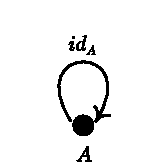
\includegraphics{./notebooks/1Cat}
    \end{center}
    \caption{Hasse diagram of Category $\bm 1$.}
    \label{fig:1Cat}
  \end{figure}
\end{example}

\begin{example}[Category $\bm 2$ and $\bm 3$]
  The Category $\bm 2$ consists of $Ob_{\bm 2} := \{A, B\}$ and $Mor_{\bm 1} = \{id_A, id_B, f\}$,
  where $f:A \to B$.
  The diagram for such Category is shown below.
  \begin{figure}[H]
    \begin{center}
      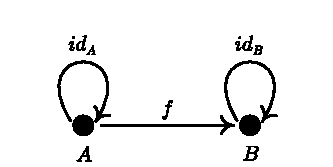
\includegraphics{./notebooks/2Cat}
    \end{center}
    \caption{Hasse diagram of Category $\bm 2$.}
    \label{fig:2Cat}
  \end{figure}

Since we know that identities are always present in Categories, we'll
omit them from future diagrams when there is no ambiguity. Thus,
the figure below represents the same diagram as Figure \ref{fig:2Cat}.
\begin{figure}[H]
  \begin{center}
    
\includegraphics{./notebooks/2Catsimple}
  \end{center}
  \caption{Hasse diagram of Category $\bm 2$ omitting identity morphisms.}
  \label{fig:2Catsimple}
\end{figure}

The Category $\bm 3$ has three morphisms besides the identities, given
by $f$, $g$ and their composition $f \fatsemi g$. The figure below
illustrates the Category with all it's morphisms.

\begin{figure}[H]
  \begin{center}
    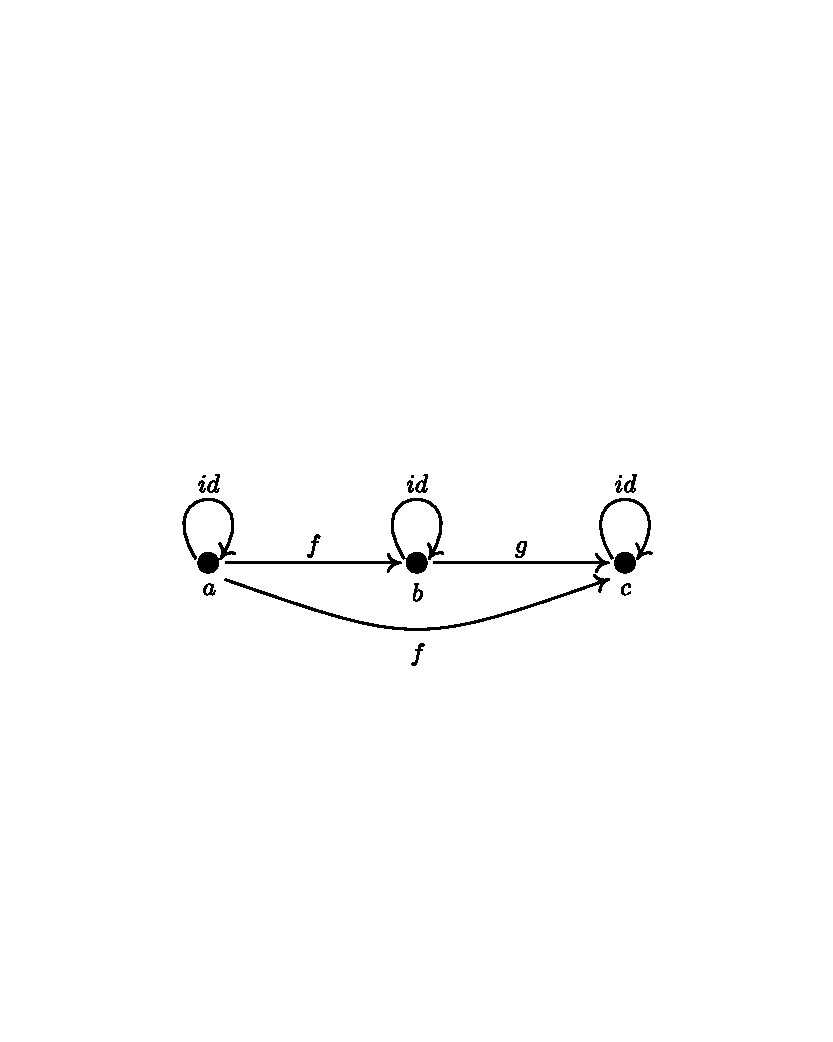
\includegraphics{./notebooks/3CatComplete}
  \end{center}
  \caption{Hasse diagram of Category $\bm 3$ showing all morphisms.}
  \label{fig:3Catcomplete}
\end{figure}

Drawing all the morphisms can make the diagram become too crowded, specially
as the number of objects and morphisms grows. Hence, we simplify the
diagram representation by ommiting not only the identity morphisms, but also
the compositions. These can always be assumed to exist, since they are a necessery
condition for every Category.
Thus, the figure below represents the same diagram as Figure \ref{fig:3Catcomplete}.

\begin{figure}[H]
  \begin{center}
    
\includegraphics{./notebooks/3Catsimple}
  \end{center}
  \caption{Hasse diagram of Category $\bm 3$ omitting identities and compositions.}
  \label{fig:3Catsimple}
\end{figure}

\end{example}

\begin{example}[Preorders]
  A Preorder is defined by a tuple $(P, \leq)$, where $P$ is a set of values, such that
  \begin{enumerate}[(i)]
    \item For $a,b \in P$, if $a\leq b$ and $b \leq c$, then $a \leq c$;
    \item For every $a \in P$, $a \leq a$.
  \end{enumerate}
  We can show that actually, this is a Category, which we'll call $\mathfrak P$,
  where $Ob_\mathfrak P = P$ and each morphism $f$ represents $a \leq b$, where
  $cod_f = a$ and $dom_f = b$.
  One example of preorder is the set of $\mathbb N$ equiped with the binary relation $\leq$
  which is shown in the diagram below.

\begin{figure}[H]
  \begin{center}
    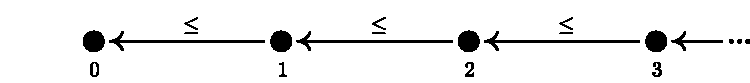
\includegraphics{./notebooks/NCat}
  \end{center}
  \caption{Hasse diagram of Preorder Category of Natural numbers.}
  \label{fig:NCat}
\end{figure}
\end{example}

Note that in preorders, there is at most one morphism between each pair of objects.
Thus, Categories with such property are often referred as \textit{thin Categories}
or \textit{preorder Category} (in \citet{fong2019invitation}, the authors call this
a \textit{preorder reflection}).

There are many other examples:
\begin{enumerate}[1.]
  \item $\bm{Set}$ which is the Category of sets, where the objects are sets and the morphisms are functions between sets.
  \item $\bm{Top}$ is the Category where topological spaces are the objects and continuous functions are the morphisms.
\end{enumerate}


\subsection{Programming with Category Theory}

One might be surprised to find out that Category Theory,
although very abstract in nature, has actual applications in the
``real world''. A very interesting example of this is in programming.

In programming languages such as Julia, we can think of `Types`
as objects and functions as morphisms.

\subsection{Isomorphism, monomorphism and epimorphism}

A very important definition in Category Theory is the notion of isomorphism.
In Set Theory, we say that two sets are isomorphic if there is an invertible
function between them. Yet, this concept is not restricted to Set Theory
and can be generalized in Category Theory as follows:

\begin{definition}[Categorical Isomorphism]
  Let $\mathcal C$ be a category with $X,Y \in Ob_\mathcal C$ and $f \in Mor_\mathcal C (X,Y)$.
  \begin{enumerate}[(i)]
    \item We say that $f$ is \textit{left invertible} if there exists $f_l \in Mor_\mathcal C (Y,X)$ such
      that $f_l \circ f = id_X$;
    \item We say that $f$ is \textit{right invertible} if there exists $f_r \in Mor_\mathcal C (Y,X)$ such
      that $f \circ f_r = id_Y$;
    \item We say that $f$ is invertible if it's both left and right invertible.
  \end{enumerate}
  When an invertible morphism exists between $X$ and $Y$, we say that they are isomorphic.
\end{definition}

\begin{proposition}
  The following properties on inverses are true:
  \begin{enumerate}[1.]
    \item If $f$ is an invertible morphism, then the left and right inverses are the same.
    \item If $f$ and $g$ are invertible and composable, then $f \circ g$ is also invertible.
  \end{enumerate}
\end{proposition}
\begin{proof}
1. Let $f$ be invertible with left inverse $f_l$ and right inverse $f_r$. Therefore,
\begin{displaymath}
  f_l \circ id_Y = f_l \circ f \circ f_r = id_X \circ f_r = f_r.
\end{displaymath}

2. Let $f:A\to B$ and $g: B \to C$ be invertible and composable, with $f\circ g: A \to C$.
There exists the inverses $g^{-1}: C \to B$ and $f^{-1}:B \to A$. Note that
$f^{-1}\circ g^{-1}:C \to A$, thus
\begin{align*}
  (f^{-1} \circ g^{-1}) \circ (g \circ f) =
  f^{-1} \circ (g^{-1} \circ g) \circ f =
  (f^{-1} \circ id_B) \circ f =
  f^{-1} \circ f =
  id_A.
\end{align*}
\begin{align*}
  (g \circ f) \circ (f^{-1} \circ g^{-1})  =
  g \circ (f \circ f^{-1}) \circ g^{-1} =
  g \circ (id_B \circ g^{-1}) =
  g \circ g^{-1} =
  id_B.
\end{align*}
We conclude that $(g\circ f)^{-1} = f^{-1} \circ g^{-1}$.
  
\end{proof}
Although similar to set isomorphism, categorical isomorphism is in a sense more general,
and captures our intuition of isomorphism between categories better than the set theoretic case,
even when we have finite objects.

Consider the following example.
Let $\mathcal P$ be the category of Posets, where posets $(P,\leq_p)$ are the objects.
Take two objects $P_1, P_2 \in Ob_\mathcal P$,
where $P_1:=\{a,b\}$ with $a$ and $b$ \textbf{not} comparable,
and $P_2:=\{0,1\}$ where indeed $0 \leq 1$. The question is whether $P_1$ is ``actually'' isomorphic
to $P_2$, and our intuition say that they should not be, since 
$P_1$ has two incomparable elements while $P_2$ has two comparable elements.

If we use the set theoretic definition, we would conclude that they \textbf{are} isomorphic,
since there is a bijective function between $P_1$ and $P_2$. 
Take for example $f:P_1\to P_2$ where $f(a)=0$ and $f(b)=1$.
So the set theoretic isomorphism does not capture what we want. What about the categorical isomorphism?
We can prove that this will not be an isomorphism using the categorical definition. Yet,
in order to prove this, we need to specify what are the morphisms between the posets,
and to do this, we need to define what are functors.

In the same way that set isomorphism is not the same as categorical isomorphism,
the notions of injectivity and surjectivity are not equivalent to their categorical
counterparts, which are called monomorphism and epimorphism.

\begin{definition}[Monomorphism]
  Let $\mathcal C$ be a category and $f \in Mor_\mathcal C(A,B)$. We say that
  $f$ is a monomorphism (or monic), if
  \begin{displaymath}
    f \circ g = f \circ h \implies g = h.  
  \end{displaymath}
\end{definition}

\begin{definition}[Epimorphism]
  Let $\mathcal C$ be a category and $f \in Mor_\mathcal C(A,B)$. We say that
  $f$ is an epimorphism (or epic), if
  \begin{displaymath}
    g \circ f = h \circ f \implies g = h.
  \end{displaymath}
\end{definition}
\textbf{Important!} A morphism $f$ can be both epic and monic, without being
an isomorphism, which again highlights the difference between this concepts and their
set-theoretic counterparts.

\begin{proposition}
  The following properties on monomorphism and epimorphism are true:
  \begin{enumerate}[1.]
    \item $f$ left-invertible $\implies$ $f$ is monic. The converse are is not true.
    \item $f$ right-invertible $\implies$ $f$ is epic. The converse are is not true.
    \item $f$ invertible $\implies$ $f$ is monic and epic. The converse are is not true.
    \item $f$ monic and right-invertible $\implies $ $f$ is isomorphism.
    \item $f$ epic and left-invertible $\implies $ $f$ is isomorphism.
  \end{enumerate}
\end{proposition}

\begin{proof}
1. Note $f:A \to B$ left-invertible implies that there exists a $f_l:B \to A$ such that
$f_l \circ f = id$. Hence, for a $g:B\to C$ and $h: B \to C$, if
\begin{displaymath}
  f \circ g = f \circ h,
\end{displaymath}
then we have that
\begin{displaymath}
  f_l \circ f \circ g = f_l \circ f \circ h \implies g =h.
\end{displaymath}
To show that the converse is false, consider the category $\mathbf{2}$(Figure \ref{fig:2Cat}). Note that
$f:A\to B$ is monic, since the only morphism that composes with $f$ is
$id_A$ and $id_B$. Yet, note that $f$ is not left invertible, since there isn't even
a morphism from $B$ to $A$.

2. Use the same argument, but reversing the order of the compositions.
For the converse, again consider the same category $\mathbf{2}$. Note that
$f:A\to B$ is epic, but it's not right invertible.

3. True since invertible means left and right invertible.

4. Since $f:A \to B$ right invertible, then there exists $f_r:B \to A$
such that $f \circ f_r = id_B$. Thus,
\begin{displaymath}
  id_B \circ f = (f \circ f_r) \circ f =
  f \circ (f_r \circ f) =
  f \circ id_A \implies f_r \circ f = id_A.
\end{displaymath}
5. Same argument.
\end{proof}

\subsection{Zero, Initial and Terminal Objects}

\begin{definition}[Zero, Initial and Terminal]
  Let $\mathcal C$ be a category.
  \begin{enumerate}[1.]
    \item An object $I \in Ob_\mathcal C$ is \textit{initial} if for every $A \in Ob_\mathcal C$,
      there is exactly one morphism from $I$ to $A$. Thus, from $I$ to $I$ there is only the identity.
    \item An object $T \in Ob_\mathcal C$ is \textit{terminal} if for every $A \in Ob_\mathcal C$,
      there is exactly one morphism from $A$ to $T$. Thus, from $I$ to $I$ there is only the identity.
    \item An object is \textit{zero} if it's both terminal and initial.
  \end{enumerate}
\end{definition}

Note that in the definitions above, we are defining these objects in terms of existence and
uniqueness of morphisms, which is known in category theory as \textbf{universal constructions}
(more on this later).

\begin{theorem}
  Every \textit{initial} object is unique up to an isomorphism, i.e. if in a category there 
  are two \textit{initial} objects, then they are isomorphic.
  Similarly, \textit{terminal} objects are unique up to an isomorphism.
\end{theorem}
\begin{proof}
  Let $I_1, I_2$ be initial. Then, there exists only $f:I_1 \to I_2$ and $g:I_2 \to I_1$.
  But since $g \circ f:I_1 \to I_1$ is a morphism from the initial object $I_1$, it must
  be equal to $id_{I_1}$. The same for $I_2$, which implies that $f$ and $g$ are inverses,
  and thus the objects are isomorphic.
  The same proof works for terminal objects.
\end{proof}


\begin{example}[Terminal and Initial Objects in $\mathbf{Set}$]
Without thinking too much, one might assumet that in the category $\mathbf{Set}$
the empty set would be a zero object; but that's not true.
In reality, the empty set is the initial object, since $f:\emptyset \to B$
is the only function from the empty set to any other set. Why is this valid?

Remember that in set theory, a function from two sets is defined as a binary
relation such that for every $x \in dom_f$, there is a unique $y \in cod_f$, i.e.
$f$ is a triple $(A,B,G)$, where $A = dom_f$, $B = cod_f$ and $G \subset A \times B$
such that $\forall x \in dom_f$, there exists a unique $y \in B$, such that $(x,y) \in G$.

Since $dom_f = \emptyset$, we have that $G \subset \emptyset \times B$, but this
is actually empty. Why? If $\emptyset \times B$ is not empty, then there exists
$(a,b) \in \empty \times B$, which is false, since this would imply that
$a \in \emptyset$, which contradicts the definition of the empty set that says
that it can have no elements (note that $\emptyset \in \emptyset$ is actually false).

With this, we have that $G = \emptyset$, thus, the only possible function from
$\emptyset$ to $B$ is $f = (\emptyset, \emptyset, B)$. Which proves that the
empty set is initial.

But what about terminal? The empty set actually does not have any morphisms
that arrives on it, since there is no function $f:A \to \emptyset$.
The terminal sets in $\mathbf{Set}$ are actually all the singletons (sets with only
one element), since for any $\{a\}$, there will be only one function
$g: A \to \{a\}$, which is $g(x) = a$.
\end{example}

Another definition we have is that of a \textit{zero} morphism. The idea here
is that this morphism must take the elements of an object $A$ to the
zero element in $B$, for example, a for two vector spaces $\mathbb R^n$ and $\mathbb R^m$,
the zero linear transformation $z:\mathbb R^n \to \mathbb R^m$ should take every vector
$n$-dimensional vector to the $\mathbf{0}$ $m$-dimensional vector. In Category
Theory we do not talk about morphisms according to how they act on the elements, but
only in the objects. So we cannot define $z$ by saying to which element it maps.
Yet, there is a way to do this in Category Theory, which gives rise to the \textit{zero} morphism
definition.
\begin{definition}[Zero Morphism]
  Let $\mathcal C$ be a category, and $0$ be a zero object.
  A morphism $z:A \to B$ is a zero morphism if there exists two morphisms
  $f:A\to 0$ and $g:0 \to B$, such that
  \begin{displaymath}
    z = g \circ f.  
  \end{displaymath}
\end{definition}
See that this makes intuitive sense. In our example, since we wish to take
$v \in \mathbb R^n$ to $0 \in \mathbb R^m$, we first take all $v$ to the zero object,
which in the category of vector spaces will be the zero vector space, i.e. $\{0\}$ the space
where $0 \in \mathbb R$ is the only element. So now all $v$ are $0$. Note that
every linear transformation from $\{0\}$ to $\mathbb R^m$ must take $0$ to $\mathbf{0} \in \mathbb R^m$,
otherwise, suppose that $g(0)=\mathbf{v} \neq \mathbf{0}$, hence for a scalar $\alpha$,
\begin{displaymath}
  g(0) = g(\alpha0) = \mathbf{v} \neq \alpha \mathbf{v} = \alpha g(0).
\end{displaymath}
This is a contradiction, since $g$ is a linear transformation.

\begin{theorem}
  Let $\mathcal C$ be a catgory with zero object $0$.
  Then there exists a unique zero morphism between any two objects.
\end{theorem}
\begin{proof}
  Let $A, B \in Ob_\mathcal C$.
  By the definition of the zero object, there exists a unique 
  $f:A \to 0$ and $g:0\to B$, thus, $g \circ f$ is a zero morphism
  by definition and is unique, since there is no other $f$ and $g$ with these respective
  domain and codamain.

  Moreover, note that if $z:A \to B$ is our zero morphism and $h:B \to C$, then
  \begin{displaymath}
    h \circ z = h \circ (g \circ f) = (h \circ g) \circ f.
  \end{displaymath}
  But, $l =(h \circ g):0 \to C$, which means that $l \circ f$ is a zero morphism.
  The same argument works with a composition from the other direction. This means
  that compositions with zero morphisms return zero morphisms.
\end{proof}

\subsection{Understanding Duality}

In several fields of Mathematics, one is faced with the informal notion of a dual.
Mathematicians define a concept, and call them the dual in some sense, for example,
the dual vector space, the dual of an optimization problem, and many more.
I always found puzzling what exactly held these things together, i.e.
what was the underlying principle that made something a dual of another.

Fortunately, Category Theory has a very elegant answer. For a given
category $\mathcal C$, the dual category is denoted by
$\mathcal C^{op}$ where are the objects are the same, but the morphisms
are inverted. This means that $Ob_{\mathcal C} = Ob_{\mathcal C^{op}}$,
and for every $f\in Mor_\mathcal (A,B)$, we have $f^{op} \in Mor_{\mathcal C^{op}}(B,A)$.

This definition gives rise to a very interesting result (observation), called the
\textit{Duality Principle}.

\begin{definition}[Dual Property and Dual Statement]
  We say $p^{op}$ is the dual property for $p$ if for all categories
  \begin{displaymath}
    \mathcal C \text{ has }p^{op} \iff
    \mathcal C^{op} \text{ has }p.
  \end{displaymath}

  For a statement $s$ about a category $\mathcal C$, the dual statement is the same
  statement, but with regards to $\mathcal C^{op}$.
\end{definition}
For example, ``a category has an initial object if and only if the dual category has a terminal object''.
In this example, the property of having an initial object is the dual property of having a terminal object,
since the above statement is true for any category.
What about the dual statement? The dual for the statement ``the category $\mathcal C$ has an initial object''
is ``the category $\mathcal C^{op}$ has an initial object''. Note that the dual statement is not always true.
And here is where we get the duality principle.

\begin{definition}[Duality Principle]
  If a statement $s$ is true for every Category, then the dual statement is also true for every
  category.
\end{definition}
Let's digest a bit what this principle states. If we can prove that a certain statement is
true for any arbitrary category, then it's dual will also be true without any effort what so ever.
\citet{roman2017introduction} gives a nice example of this. We already prove that for any
category, if an initial object exists, this initial object is unique up to an isomorphism.
Note that this is a statement that is true for any category, so the duality principle applies,
i.e. the dual statement is true. And what is the dual statement? That for every $\mathcal C^{op}$
the initial object is unique up to an isomorphism. But an initial object in $\mathcal C^{op}$
is a terminal object in $\mathcal C$. So we have, without any effort, that every terminal
object is unique up to an isomorphism.



\section{Functors}
Another central definition in Category Theory is that of Functors.
While morphisms relate objects inside a Category, a Functor
establishes a relation between Categories, thus, it's one level
higher in terms of abstraction.


\subsection{What is a Functor?}

Let's formally define a Functor.

\begin{definition}[Functor]
  Let $\mathcal C$ and $\mathcal D$ be two Categories. A functor $F: \mathcal C \Rightarrow \mathcal D$ is
  a pair of mappings with the following properties:
  \begin{enumerate}[(i)]
    \item a mapping between objects
      \begin{displaymath}
        F:Ob_\mathcal C \to Ob_\mathcal D,
      \end{displaymath}
      where for each $A \in Ob_\mathcal C$, $F(A) \in Ob_\mathcal D$.
    \item a mapping between morphisms
      \begin{displaymath}
        F:Mor_\mathcal C \to Mor_\mathcal D,
      \end{displaymath}
      where there are two possibilities:
      \begin{enumerate}
        \item \textbf{Covariant Functor}, in which
          \begin{displaymath}
            F:Mor_\mathcal C(A,B) \to Mor_\mathcal D (F(A),F(B)),
          \end{displaymath}
          hence for a morphism $f:A \to B$, then $F(f):F(A) \to F(B)$.
        \item \textbf{Contravariant Functor}, in which
          \begin{displaymath}
            F:Mor_\mathcal C(A,B) \to Mor_\mathcal D (F(B),F(A)),
          \end{displaymath}
          hence for a morphism $f:A \to B$, then $F(f):F(B) \to F(A)$.
      \end{enumerate}
    \item Identities morphisms are preserved, i.e. for $A \in Ob_\mathcal C$
        \begin{displaymath}
          F(id_A) =  id_{F(A)}.
        \end{displaymath}
    \item Compositions are preserved, i.e. for $f \in Mor_\mathcal C(A,B)$
      and $ g \in Mor_\mathcal C(B,C)$,
      \begin{enumerate}
        \item For a \textbf{Covariant Functor},
          \begin{displaymath}
            F(f \circ g) = F(f) \circ F(g).
          \end{displaymath}
        \item For a \textbf{Contravariant Functor},
          \begin{displaymath}
            F(f \circ g) = F(g) \circ F(f).
          \end{displaymath}
      \end{enumerate}
  \end{enumerate}
  It's common for authors to refer to covariant functors only as functors, i.e.
  whenever someone say that $F$ is a functor, it might be implied that it's a covariant functor.
  We'll also use this convention whenever it's not ambiguous, and we'll always.
  Also, we'll sometimes use $FA$ to mean $F(A)$.
\end{definition}

Again, the use of diagrams may help understand what is going on. The figure below
illustrates the identity and composition preservation of Functors.

\begin{figure}[H]
  \begin{center}
    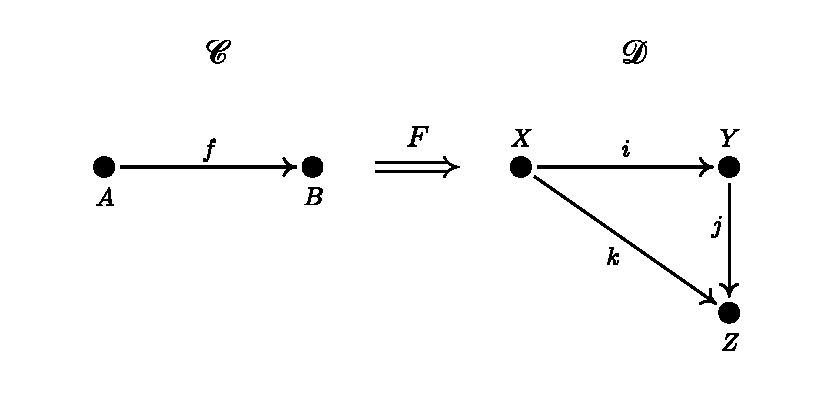
\includegraphics[width=1.1\textwidth]{./notebooks/Functor.pdf}
  \end{center}
  \caption{Diagrams showcasing the properties of Functors.}
  \label{fig:Functor}
\end{figure}

\subsection{Category of Small Categories}

One might realize that functors are acting on Categories in a very similar way as morphisms
do to objects. Indeed, we can define a functor composition to be
such that for two functors $F:\mathcal C \Rightarrow \mathcal D$
and $G:\mathcal D \Rightarrow \mathcal E$, then $G \circ F$ is
a functor from $\mathcal C$ to $\mathcal E$ where
\begin{enumerate}
  \item For any $A \in Ob_\mathcal C$, $G\circ F (A) = G(F(A))$,
  \item For any $f \in Mor_\mathcal C$, $G\circ F (f) = G(F(f))$.
\end{enumerate}
We can also define an identity functor $I:\mathcal C \Rightarrow \mathcal C$,
where $F(A) = A$ and $F(f) = f$.

Therefore, we might wonder whether there exists a Category of all Categories
where objects are Categories and morphisms are functors.
The answer is ``no''. Similar to the set of all sets, it can be proven
that this Category does not exists. Yet, the Category of all \textit{small Categories}
does.

Remember, a small Category is one where both morphisms and objects are sets.
With this, let's prove our first theorem.
\begin{theorem}[Category of Small Categories]
  Let $Ob_{\textbf{SmCat}}$ be small Categories and $Mor_{\textbf{SmCat}}$ be functors.
  This constitutes a Category.
\end{theorem}
\begin{proof}
  To prove this, we'll use the fact that in Gödel-Bernays class set theory, the
  axiom \ref{axiom:gb} implies what is called a \textit{comprehension scheme}.
  \begin{proposition}[Comprehension Scheme from \citet{borceux1994handbook}]
    If $\phi(x_1,...,x_n)$ is a formula that the quantification occurs on set variables, then
    there exists a class $A$ such that
    \begin{displaymath}
      (x_1,...,x_n) \in A \iff \phi(x_1,...,x_n).
    \end{displaymath}
  \end{proposition}
  Note that
  \begin{displaymath}
    \mathcal C := \langle Ob_\mathcal C, Mor_\mathcal C \rangle \in \textbf{SmCat} \iff
    \mathcal C \text{ ``is a Category''}.
  \end{displaymath}
  Since every $\mathcal C$ is small, then the formula to check whether $\mathcal C$ is a Category
  iterates over set variables, i.e. $Ob_\mathcal C$ and $Mor_\mathcal C$.
  Thus, the Comprehension Scheme proposition guarantees that $\textbf{SmCat}$ exists.
\end{proof}

\subsection{Types of Functors}

Before we go on to provide examples of functors, let's present
a way to classify different functors.

\begin{definition}[Faithful, Full, Fully Faithful and Embedding]
  Here we follow \citet{roman2017introduction}.
  Let $F$ be a functor between categories $\mathcal C$ and $\mathcal D$.
  \begin{enumerate}[1.]
    \item $F$ is \textbf{faithful} if for every $A,B \in Ob_\mathcal C$,
      $F:Mor_\mathcal C(A,B)\to Mor_\mathcal C(FA,FB)$ is injective.
    \item $F$ is \textbf{full} if for every $A,B \in Ob_\mathcal C$,
      $F:Mor_\mathcal C(A,B)\to Mor_\mathcal C(FA,FB)$ is surjective.
    \item $F$ is \textbf{fully faithful} if for every $A,B \in Ob_\mathcal C$,
      $F:Mor_\mathcal C(A,B)\to Mor_\mathcal C(FA,FB)$ is bijective.
    \item $F$ is an \textbf{embedding} of $\mathcal C$ in $\mathcal D$ if $F$ is fully faithful
      and $F:Ob_\mathcal C \to Ob_\mathcal D$ is injective.
  \end{enumerate}
 
\end{definition}

\subsection{Subcategories}

\begin{definition}[Subcategory]
  Let $\mathcal D$ be a category. We say that $\mathcal C$
  is a subcategory of $\mathcal D$ if $Ob_\mathcal C \subset Ob_\mathcal D$ and
  $Mor_\mathcal C \subset Mor_\mathcal D$, such that $\mathcal D$ is a category.

  If for every $A, B \in Ob_\mathcal D$, we have that $Mor_\mathcal D (A,B) = Mor_\mathcal C(A,B)$,
  then $\mathcal D$ is a \textit{full subcategory}.
\end{definition}

From the definition of a functor, one might wonder whether for any
functor $F:\mathcal C \Rightarrow \mathcal D$,
the image $F(\mathcal C)$ is a subcategory of $\mathcal D$, i.e.
if $\langle Ob_{F(\mathcal C)}, Mor_{F(\mathcal C)} \rangle$ is a category where
\begin{displaymath}
  Ob_{F(\mathcal C)}:= \{F(A) : A \in Ob_\mathcal C\}, \quad
  Mor_{F(\mathcal C)}:= \{F(f) : f \in Mor_\mathcal C\}.
\end{displaymath}
The answer is no.


\section{Free Categories and $\mathcal C$-Sets}

